\documentclass[main.tex]{subfiles}

\begin{document}
	\section{Reciprocal lattice and scattering} \label{seq:scattering}
	\subsection{Theory}
	The reciprocal lattice is an incredibly useful construct, as it allows for an easy description of wave phenomena, where the main variable is the wave vector $ \V{k} $. The reciprocal lattice is a lattice (as defined in the previous section), but in reciprocal space. This again means that the free variables is not position, but the wave vector.
	
	The definition of a reciprocal lattice is all of the points $ \V{G} $, that satisfy
	\begin{equation}\label{eq:reciprocal_lattice}
		e^{i \V{G} \D \V{R}} = 1,
	\end{equation}
	for any lattice point in real space $ \V{R} $. Further, the primitive lattice vectors of the reciprocal lattice all satisfy the property
	\begin{equation}\label{eq:rec_prim_def}
		\V{a}_i \D \V{b}_j = 2\pi \delta_{ij},
	\end{equation}
	where $ delta_{ij} $ is the familiar Kronecker delta. This property of the reciprocal lattice vectors is what makes $ \V{G} $ a lattice in reciprocal space. The real space lattice points have the coordinates $ \V{R} = n_1 \V{a}_1 + n_2 \V{a}_2 + n_3 \V{a}_3 $, and say an arbitrary point in the reciprocal space is constructed as
	\begin{equation}\label{eq:rec_lat_vec}
		\V{G} = m_1 \V{b}_1 + m_2 \V{b}_2 + m_3 \V{b}_3,
	\end{equation}
	then plugging these into Eq. \eqref{eq:reciprocal_lattice} we get
	\begin{equation}
		e^{i (n_1 \V{a}_1 + n_2 \V{a}_2 + n_3 \V{a}_3) \D (m_1 \V{b}_1 + m_2 \V{b}_2 + m_3 \V{b}_3)} = e^{2\pi i (n_1 m_1 + n_2 m_2 + n_3 m_3)},
	\end{equation}
	where the second equality follows from the defining property of the primitive lattice vectors in reciprocal space. For $ \V{G} $ to be part of the reciprocal lattice, for any choice of integer $ n_i $, then $ m_i $ need also be integers. As such the form of the reciprocal lattice matches that of the real space lattice. Usually (in the case of lattice planes and scattering) we express the 3 coefficients for the reciprocal lattice vectors using Miller indices ($ hkl $), where $ m_1=h, m_2 = k, m_3 = l $.
	
	Now, to actually construct the reciprocal primitive lattice vectors, the following formulas are used:
	\begin{equation}\label{eq:rec_prim_vec}
		\V{b}_1 = \frac{2\pi \, \V{a}_2 \times \V{a}_3}{\V{a}_1 \D (\V{a}_2 \times \V{a}_3)}, \quad \V{b}_2 = \frac{2\pi \, \V{a}_3 \times \V{a}_1}{\V{a}_2 \D (\V{a}_3 \times \V{a}_1)}, \quad \V{b}_3 = \frac{2\pi \, \V{a}_1 \times \V{a}_2}{\V{a}_3 \D (\V{a}_1 \times \V{a}_2)},
	\end{equation}
	where the cross product in the numerator ensures the property of the Kronecker delta, and the denominator serves as a sort of normalization, such that the dot product equals 2$ \pi $. Further, by dimensional analysis, $ \V{b}_i $ has dimensions $ \e{m}\inverse $, as expected for wave vectors.
	
	The reciprocal lattice can also be understood in terms of families of lattice planes. First, a lattice plane is defined as any plane that contains at least 3 lattice points (this also guarantees that an infinite set of lattice points is contained by the plane, by virtue of the non-uniqueness of the primitive lattice vectors). 
	
	A family of lattice planes is an infinite series of parallel planes, equally spaced, such that all points of the lattice is contained in the planes, and that all planes contain lattice points.
	
	First consider the series of planes containing the points $ \V{r}_m $, defined by
	\begin{equation}
		\V{G} \D \V{r}_m = 2\pi m,
	\end{equation}
	for some integer $ m $. This form ensures that all lattice points are contained in the planes. The minimum distance between planes can then be calculated from
	\begin{equation}
		\V{G} \D (\V{r}_2 - \V{r}_1) = 2\pi,
	\end{equation}
	as the minimum distance will be when $ (\V{r}_2-\V{r}_1) $ and $ \V{G} $ are parallel, yielding
	\begin{equation}
		d = \frac{2\pi}{|\V{G}|}.
	\end{equation}
	Now any reciprocal lattice vector will give yield a set of equidistant, parallel planes, but not all of these sets will be families of lattice planes. The family of lattice planes in the direction $ \U{G} $ will have have some distance $ d = 2\pi /|\V{G}| $, where $ \V{G} $ is a reciprocal lattice vector. An infinite set of reciprocal lattice vectors share this direction, but increasing the magnitude of the reciprocal lattice vector $ \V{G} $ will decrease the distance between the set of planes, and at some point there will be planes that do not contain any lattice points.
	
	As such, there is some minimum magnitude of the reciprocal lattice vector that defines a given family of lattice planes. This means that for a family of lattice planes, the distance is $ d = 2\pi /| \V{G}_{min}| $.
	
	\subsubsection{The Brillouin zone}
	In the one dimensional tight binding example, any plane wave with wave vector $ k $ and $ k + G_m = k + 2\pi m/a $ are physically equivalent. The wave vector is only defined up to a factor of $ 2 \pi / a $. This means that the wave vector can be chosen in the interval $ -\pi /a \leq k \leq \pi/a $, which is called the first Brillouin zone.
	
	The same principle applies to higher dimensions. The first Brillouin zone is defined as any point $ \V{k} $ in reciprocal space, that is closer to $ \V{0} $ than any other point on the reciprocal lattice. The $ n $'th Brillouin zone is then defined as any point $ \V{k} $, where $ \V{0} $ is the $ n $'th nearest point on the reciprocal lattice.
	
	For a 2 dimensional, square lattice the first Brillouin zone corresponds to a square with sides $ 2\pi /a $, centred on the origin.
	
	\subsubsection{Scattering}
	In a scattering experiment, an incoming collection of waves (be it an electrons, neutrons, x-ray photons or something completely different) with wave vector $ \V{k} $ is incident upon a crystal. Some of these will be scattered into states with wave vector $ \V{k}' $ whilst others will pass on through. 
	
	To find the general conditions for scattering, we start with Fermi's Golden Rule \cite{simon}, which is a measure of the transition rate between states. It is given as
	\begin{equation}\label{eq:Scat_fermi}
		\Gamma(\V{k}', \V{k}) = \frac{2\pi}{\hbar}|\braket{\V{k}' | V | \V{k}}|^2 \delta(E_{\V{k}'}-E_{\V{k}}),
	\end{equation}
	where the matrix element is
	\begin{equation}\label{eq:Scat_mat_el_initial}
		\braket{\V{k}' | V | \V{k}} = \infint \frac{e^{-i \V{k}'\D\V{r}}}{\sqrt{L^3}} V(\V{r}) \frac{e^{i \V{k}\D\V{r}}}{\sqrt{L^3}} \ud \V{r} = \frac{1}{L^3} \infint e^{-i(\V{k}'-\V{k}) \D \V{r}} \, V(\V{r}) \ud \V{r}.
	\end{equation}
	This is just the Fourier transform of the potential! Further, we assume the potential is periodic in the unit cell, such that $ V(\V{r} + \V{R}) =  V(\V{r}) $ for any lattice point $ \V{R} $. With this, we can define $ \V{r} = \V{R} + \V{x} $ where $ \V{x} $ is a position within the unit cell, and then split up the integral into an infinite sum over lattice points:
	\begin{equation}\label{eq:Scat_mat_el}
		\braket{\V{k}' | V | \V{k}} = \frac{1}{L^3}\infint e^{-i(\V{k}'-\V{k})\D(\V{R}+\V{x})} V(\V{R}+ \V{x}) \ud \V{x} = \frac{1}{L^3} \sum_{\V{R}} e^{-i(\V{k}'-\V{k}) \D \V{R}}\int_{\substack{\text{unit-} \\\text{cell}}} e^{-i (\V{k}'-\V{k}) \D \V{x}} V(\V{x}) \ud \V{x}.
	\end{equation}
	Now, this sum of complex exponentials has two possible outcomes. If $ \V{k}'-\V{k} $ is a reciprocal lattice vector, all the terms are unity and the sum adds up to the total number of unit cells in the crystal. If $ \V{k}'-\V{k} $ is not a reciprocal lattice vector, then the terms will just oscillate, like roots of unity, summing to 0. This condition is called the Laue condition:
	\begin{equation}\label{eq:Scat_Laue}
		\V{k}' - \V{k} =  \V{G}.
	\end{equation}
	
	Furthermore, when the scattered wave leaves the crystal, it has to have the same magnitude of the wave vector as the incoming wave, as required from the delta function in Fermi's Golden Rule:
	\begin{equation}\label{eq:Scat_E_cons}
		|\V{k}'| = |\V{k}|.
	\end{equation}
	Together these two conditions are statements of conservation of crystal momentum (\textbf{BUT WHY?}) and energy respectively.
	
	These are the two conditions for scattering on a crystal, but what about the scattering amplitudes? This is where the integral in Eq. \eqref{eq:Scat_mat_el} comes in. It turns out that the intensity of the scattered wave vector is proportional to the absolute square of this integral, called the \textit{structure factor}: \cite{simon}
	\begin{equation}
		I \propto |S(\V{G})|^2, \quad S(\V{G}) = \int_{\substack{\text{unit-} \\\text{cell}}} e^{-i (\V{k}'-\V{k}) \D \V{x}} V(\V{x}) \ud \V{x}.
	\end{equation}
	This is as far as is workable without specifying the form of the potential. For now we will assume we are working with neutron scattering. Since neutrons are not charged, they only scatter from the atomic cores by the nuclear force, and not from electrons. For this reason we model the potential of each atom in the unit cell as a delta function with some appropriate potential strength associated:
	\begin{equation}\label{eq:Scat_neutron_pot}
		V(\V{x}) \sum_{\text{atoms} \,j} f_j \delta(\V{x}-\V{x}_j),
	\end{equation}
	where the potential strength is called the \textit{form factor}. With this potential, the structure factor becomes
	\begin{equation}\label{eq:Scat_struct}
		S(\V{G}) = \sum_{\text{atoms} \,j} f_j e^{i \V{G} \D \V{x}_j}.
	\end{equation}
	
	For the purposes of the program, we will further restrict the available lattice to a simple cubic with a basis. This will allow us to illustrate the core ideas of scattering whilst keeping any clutter to a minimum.
	
	One thing this allows us to show is systemic absences. For a cubic lattice with a basis, the structure factor becomes
	\begin{equation}\label{eq:Scat_struct_ortho}
		S(\V{G}) = S_{hkl} = \sum_{\text{atoms}\, j} f_j e^{i (h\V{b}_1 + k\V{b}_2 + l\V{b}_3) \D \V{x}_j} = \sum_{\text{atoms}\, j} f_j e^{2\pi i (hx_j + ky_j + lz_j)}
	\end{equation}
	where the coordinates of $ \V{x}_j $ are in units of the lattice constant $ a $. For a bcc lattice, which corresponds to a simple cubic lattice, with two identical atoms at $ (0,0,0) $ and $ (1/2, 1/2, 1/2) $ (in units of the lattice constant), the structure factor becomes
	\begin{equation}
		S_{hkl} = f\ (1 + e^{2\pi i (h/2 + k/2 + l/2)}) = f\ (1 + e^{\pi i (h+k+l)}) = f \ (1+ (-1)^{h+k+l}),
	\end{equation}
	meaning that for there to be any scattering for a bcc lattice, $ h+k+l $ must be even. This is what is known as a systemic absence. There is also a systemic absence for fcc lattices, which can be thought of as a simple cubic lattice, with identical atoms at $ (0,0,0), (1/2, 1/2, 0), (1/2, 0, 1/2) $ and $ (0, 1/2, 1/2) $:
	\begin{equation}
		S_{hkl} = f\ (1 + e^{\pi i (h+k)} + e^{\pi i (k+l)} + e^{\pi i (h+l)}).
	\end{equation}
	Here all of $ h+k, k+l $ and $ h+l $ must be even, corresponding to $ h,k,l $ all being either even or odd. As such there are systemic absences in both bcc and fcc lattices, but not simple cubic lattices, where all combinations of $ h,k $ and $ l $ can lead to scattering.
	
	\subsection{Implementation}	
	The scattering program creates two figures. One interactive figure with the physical setup, including the desired crystal structure, incoming probe beam, detector screen and detected scattering events. The second shows only a top down view of the detector screen with the detected scattering events.
	
	For the first figure, the scattering program builds upon the lattice plotting program. It plots the desired lattice (simple cubic with a basis), calculates scattering for this crystal given a list of form factors and an incoming wave, and displays the results on a simulated detection screen.
	
	Calculating the actual scattering is done by first creating the reciprocal lattice with Eq. \eqref{eq:rec_prim_vec}, and next creating an array of reciprocal lattice vectors with indices $ h,k,l \in [-5, -4, \dots, 5] $ (excluding $ h=k=l=0 $ as this just results in a "scattered" wave vector equal to the incident wave vector). This of course does not constitute the whole possible range reciprocal lattice vectors, but a line has to be drawn somewhere. This interval includes $ 11^3 - 1 = 1330$ different reciprocal lattice vectors, which should be plenty to get an understanding of scattering.
	
	This array of reciprocal lattice vectors is then used to calculate the "scattered" wave vectors by Eq. \eqref{eq:Scat_Laue}. These do not necessarily meet the other criteria of energy conservation, though, and there are further criteria to consider. First is of course any systemic absences. These wave vectors do meet the criteria of both conservation of crystal momentum and energy, but they still do not show up on the detection screen due to the systemic absence.
	
	To calculate the systemic absence of a scattered wave vector, the structure factor for a given reciprocal lattice vector has to be calculated. This is done with Eq. \eqref{eq:Scat_struct}. Next the program calculates the intensity $ I_{hkl}=|S_{hkl}|^2 $ and checks if it is equal to 0. If so, then the scattered wave vector is subject to a systemic absence.
	
	The second additional criteria is the direction of the scattered wave vector. The scattered wave vector has to point in the direction of the detection screen, otherwise it will not physically "hit" the screen. In the program the detection screen is placed parallel to the $ xy $-plane, with $ z=5 $. As such any scattered wave vector will need to have $ k'_z > 0 $ to be detected.
	
	These three criteria (conservation of energy, lack of systemic absence, and proper direction) are all calculated by the program, and if a scattered wave vector does not fulfil all of them, it is discarded.
	
	Left are only a handful, if any, of scattered wave vectors. For each of these, the impact point of the scattered wave vector on the detection plane has to be calculated. This is done by calculating the intersection between a line and a plane. The line is defined by the point of impact $ \V{p}_0 $ of the incident wave vector along with the scattered wave vector $ \V{k}' $. The plane is defined as mentioned above, with $ z=3 $. In this case the intersection happens when
	\begin{equation}
		p_{0,z} + t\D k'_z = 3,
	\end{equation}
	for some value of $ t $. This value of $ t $ can then be used to calculate the point of intersection as
	\begin{equation}
		\V{p} = \V{p}_0 + t \V{k}'.
	\end{equation}
	These points are then plotted in the first figure along with the detection plane and the incoming wave vector (scaled so its length is equal to the wavelength).
	
	The points are also shown on the second figure, showing the top down view of the detection plane, along with the Miller indices of the reciprocal lattice vector giving rise to the corresponding scattering events.
	
	Two additional features for the scattering program are available. The first is the "show all" feature. This plots all outgoing wave-vectors and their associated lines (starting at the impact point for the incident beam, and ending at the intersection between the outgoing wave vector and the detection plane).
	
	The second is a "highlighting" feature. This feature works by taking a set of Miller indices and highlighting the scattering associated with said set (if scattering occurs for this reciprocal lattice vector). It plots the relevant scattering event in a different colour, and plots the associated lattice planes.
	
	These planes are created in one of two ways. If the plane is \textit{not} perpendicular to the $ xy $-plane (corresponding to a normal vector $ \V{n} $ with a $ z $-component different from 0) the equation of the plane is used with the origin as the starting point $ \V{r}_0 $. For the normal vector, the program uses the displacement vector $ \V{d} = 2\pi \U{G} / |\V{G}| $:
	\begin{equation}
		0 = \V{d} \D (\V{r}-\V{r}_0) = \V{n} \D \V{r}, \quad \Leftrightarrow \quad z = -\frac{d_x x + d_y y}{d_z}.
	\end{equation}
	The program then calculates the $ z $-component of the plane from a given array of $ x $ and $ y $-values. This, of course, only creates one plane. Each subsequent plane is created by displacing the original plane by an amount $ d/\cos \theta = d^2/d_z$. This process is repeated in the positive direction until the smallest $ z $-value of the uppermost plane is outside of the plot box, and likewise in the negative direction, yielding a full set of parallel planes, spaced by $ \V{d} $ (at least within the plot box).
	
	However, if the plane \textit{is} perpendicular to the $ xy $-plane, this method does not work. Here the program creates a plane from the span of two vectors perpendicular to the displacement vector. Since the plane is perpendicular to the $ xy $-plane, one such vector is $ \U{z} $, the unit vector in the $ z $-direction. Then the second vector can just be taken as the cross product between $ \V{d} $ and $ \U{z} $. Again the origin is taken as the starting point:
	\begin{equation}
		\V{r} = \V{r}_0 + s \U{z} + t (\U{z} \times \V{d}).
	\end{equation}
	To get any subsequent planes, an integer multiple of the displacement vector $ \V{d} $ is added to the starting plane.
	
	For both of these methods the planes need to be limited so they are only plotted within the plot box. This is done by replacing the $ z $-component of any point outside the plot box with \texttt{NaN}, which will cause Matplotlib to not plot the associated point. This is especially pertinent in the second case, where not only the $ z $-component can be outside the plot box, but $ x $ and $ y $-components can be. Because of this $ \U{z}/4 $ and $ (\U{z} \times \U{G})/4 $ are used to increase the resolution of each plane, along with a large range of values for $ s $ and $ t $ (in this case taken to be integers, though the same effect could be achieved by using a more densely packed interval for $ s $ and $ t $ and keeping the original vectors).
	
	 
	Further, a second program is added alongside the scattering program. This second program just allows the user to plot any crystal, along with any set of lattice planes, defined by a set of Miller indices supplied by the user.
	
	\subsection{Examples}
	\begin{wrapfigure}{r}{2in}
		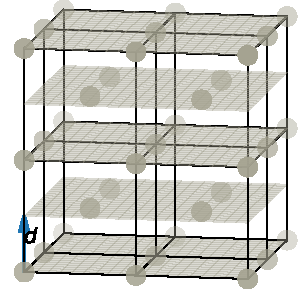
\includegraphics[width=2in]{figures/lattice_planes_1.pdf}
		\caption{A bcc lattice showing the (001) family of lattice planes.}
		\label{fig:lattice_planes}
	\end{wrapfigure}
	Say we want to simulate neutron scattering on a cubic lattice with a four atom basis (one at lattice points, the others at the centre of the faces of the unit cell). We set the relative scattering lengths as 1 for the atoms on the lattice points and 0.5 for the others. We set $ \V{k}_{in} = (0, 0, -1.5)$ in units of $ 2\pi/a $. Lastly we highlight the scattering corresponding to the Miller indices (112). This is all done by the following line, and produces figure \ref{fig:scattering_no_systemic}.
\begin{lstlisting}
Scattering(k_in=np.array([0, 0, -1.5])
		   basis=np.array([[0, 0, 0], 
						   [0.5, 0.5, 0],
						   [0.5, 0, 0.5],
						   [0, 0.5, 0.5]]),	
		   highlight=(1,1,2)
		   scattering_length=np.array([1, 0.5, 0.5, 0.5]))
\end{lstlisting}

	If instead we want to plot scattering on regular fcc lattice, with the same wave vector, we just set the scattering length for all atoms to 1. This gives figure \ref{fig:scattering_systemic}.
\begin{lstlisting}
Scattering(k_in=np.array([0, 0, -1.5])
		   basis=np.array([[0, 0, 0], 
						   [0.5, 0.5, 0],
						   [0.5, 0, 0.5],
						   [0, 0.5, 0.5]]),	
		   scattering_length=np.array([1, 0.5, 0.5, 0.5]))
\end{lstlisting}
	As a last example, say we just want to plot the (001) family of lattice planes for a bcc lattice, then we write the following and get figure \ref{fig:lattice_planes}.
\begin{lstlisting}
Reciprocal(lattice_name="bcc",
		   indices=(0,0,1))
\end{lstlisting}
	
	
	\begin{figure}
		\centering
		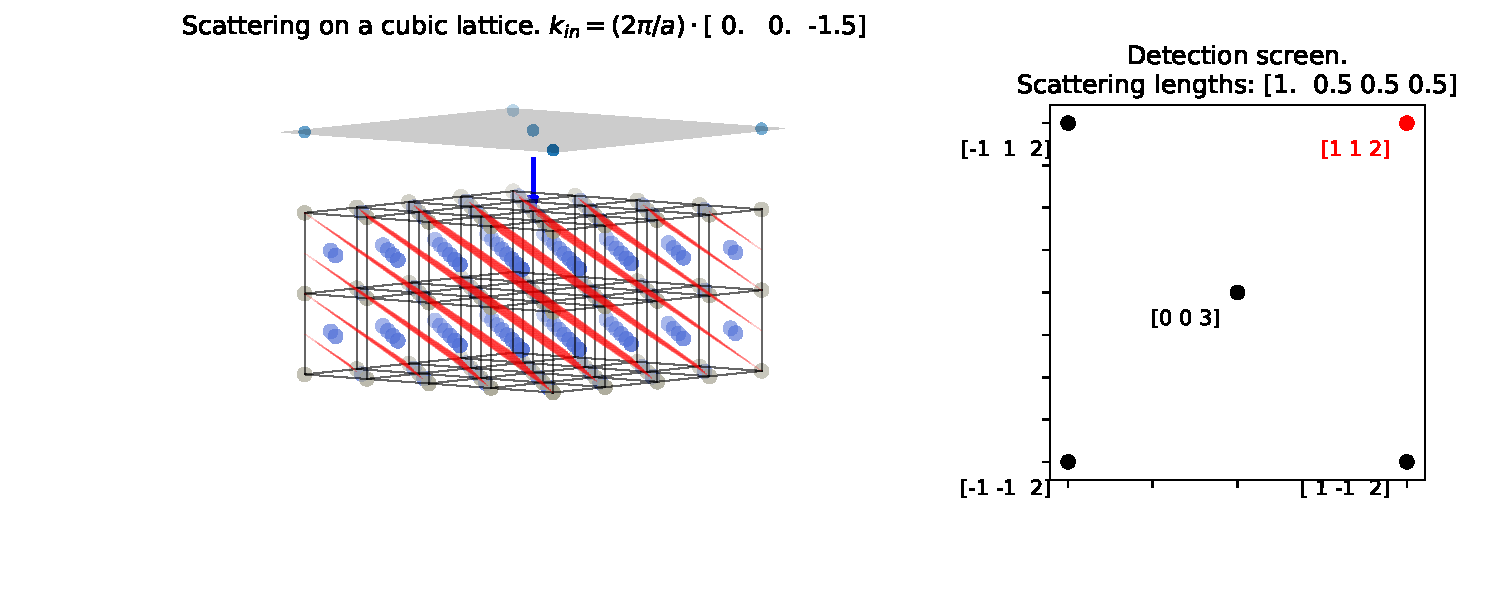
\includegraphics[width=\linewidth]{figures/scattering_no_systemic.pdf}
		\caption{Scattering on a cubic lattice with a four atom basis (one at lattice points and the others on the faces of the unit cell), with form factors of 1 for the lattice point atoms, and 0.5 for the others. The choice of incoming wave vector gives rise to 5 scattering events, corresponding to 5 different sets of miller indices. Note the highlighted point and associated family of planes. They are not lattice planes, which means that for a proper fcc lattice, this set of Miller indices will be subject to systemic absence.}
		\label{fig:scattering_no_systemic}
	\end{figure}

	\begin{figure}
		\centering
		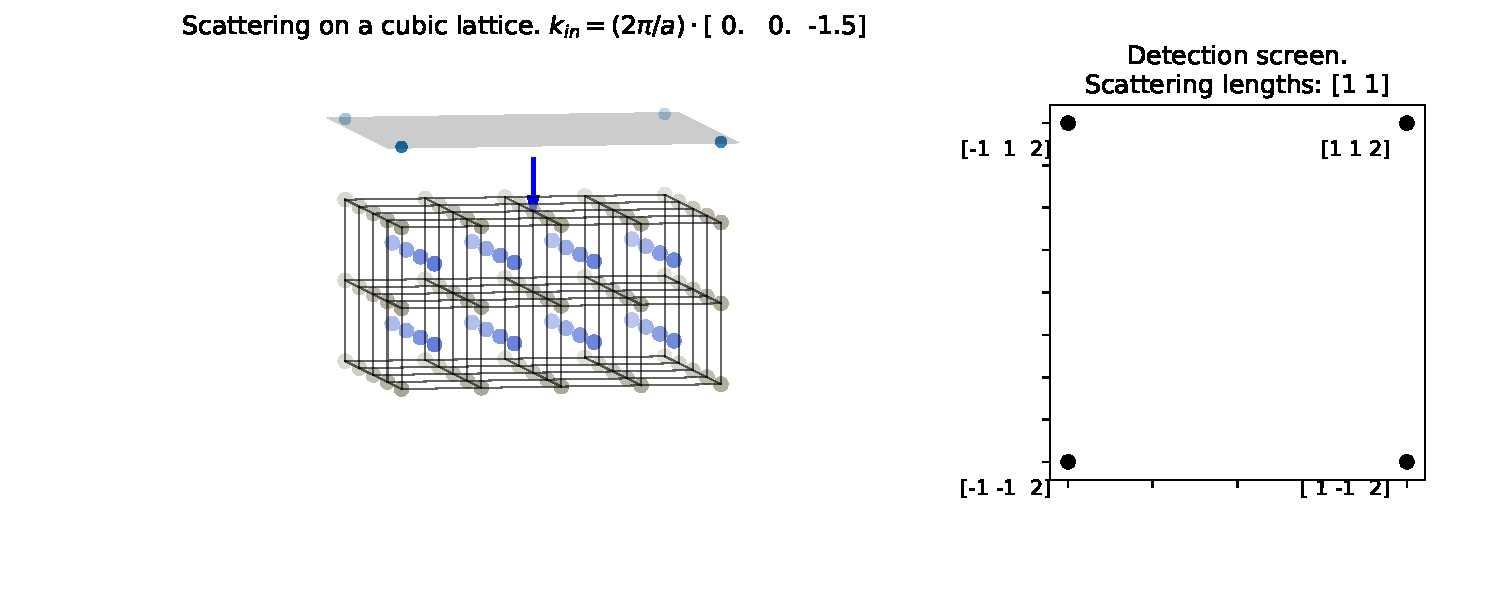
\includegraphics[width=\linewidth]{figures/scattering_systemic.pdf}
		\caption{The same scattering setup as in figure \ref{fig:scattering_no_systemic}, but with equal form factors for the four atoms (effectively an fcc lattice). Note the absence of scattering events due to systemic absence, since for each of the sets of Miller indices either $ h+k $, $ k+l $ or $ h+l $ is odd.}
		\label{fig:scattering_systemic}
	\end{figure}

	

\end{document}